%%%%%%%%%%%%%%%%%%%%%%%%%%%%%%%%%%%%%%%%%%%%%%%%%%%%%%%%%%%%%%%%%%%%%%%%%%%%%
%	e-Yantra, IIT-Bombay

%	Document Author: Abhishek Rathore, Gopineedi Harsha Vardhan
%	Date: 07-June,2016 

%%%%%%%%%%%%%%%%%%%%%%%%%%%%%%%%%%%%%%%%%%%%%%%%%%%%%%%%%%%%%%%%%%%%%%%%%%%%%

\documentclass[11pt,a4paper]{article}

\usepackage{graphicx}
\usepackage{listings}
\usepackage{url}
\usepackage{float}
\usepackage{subcaption}
\title{Object Tracking (Based on ROI)}
\author{e-Yantra Team}
\date{\today}

\begin{document}
	\maketitle
	\newpage
	\tableofcontents
	\newpage
	\section{Object Tracking (Based on ROI)}
	The objective of this tutorial is to track an object(or some region) by giving a Region Of Interest(ROI)using a mouse to the module .We track the object/region by using algorithms like Meanshift and CAMshift techniques.
	\section{Prerequisites}
	User should have handy knowledge of following before reading this tutorial.
	\begin{itemize}
		\item Basics of Python Language.
		\item Introduction to OpenCV.
		\item Basics of Image processing in OpenCV using Python.
		\item Knowledge on Mean Shift Algorithm,Histograms and Back projections.
	\end{itemize}
	\section{Hardware Requirement}
	\begin{itemize}
		\item A Computer with internal or external webcam.
	\end{itemize}
	\section{Software Requirement}
	\begin{itemize}
		\item Python 2.7.5 (with OpenCV and Numpy module)
		\item OpenCV 2.4.9 
		\item numpy 1.7.1
		\item Any sample video(that can be used for object tracking)
		\item \textbf{Note :} These versions I had at the time of this tutorial.
	\end{itemize}
	\section{Theory and Description}
	\begin{itemize}
		\item Here we track the objects using color probability distribution.We consider the hue and saturation values(can also be done considering only hue value) and find their values in each pixel of the ROI .(taken from first frame)
		\item We track the objects by converting the ROI frame into Histograms and using back projection on the histogram we can vary the object from the background(like masking a colored object)
		\item After getting the back projection of the Object ,we use different algorithms like Mean and CAM Shift for tracking the object in the following frames
		\begin{figure}[h!]
			\includegraphics[scale=0.5 ]{original.jpg}
			\centering
			\caption{Sample Image}
		\end{figure}
		\begin{figure}[h!]
			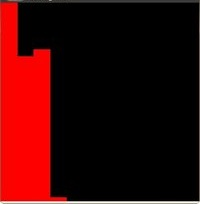
\includegraphics[scale=0.5 ]{Histogram.jpg}
			\centering
			\caption{Histogram}
		\end{figure}
		\begin{figure}[h!]
			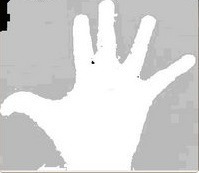
\includegraphics[scale=0.5 ]{BackProjection.jpg}
			\centering
			\caption{Back Projection}
		\end{figure}
		\item Same process works in each frame and we track the colored object.
		\item \textbf{Note :} Camshift and Meanshift may not work properly when there is a similar colored object in the frame as we had taken hue and saturation values for tracking.
		\newpage
		\textbf{Algorithms used:}
	\vspace{0.2cm}
	\subsection{Mean Shift Algorithm}
	\begin{itemize}
	 \item Mean shift is a non-parametric feature-space analysis technique, a so-called mode seeking algorithm. It is a procedure for locating the maxima of a density function given discrete data sampled from that function. In a sense, it is using a non-parametric density gradient estimation. It is useful for detecting the modes of this density.
	 \item Moving objects are characterized by their color-histograms. Therefore the key operation of the object tracking algorithm is histogram estimation. Mean-shift tracking algorithm is an iterative scheme based on comparing the histogram of the original object in the current image frame and histogram of candidate regions in the next image frame. 
	  \item The aim is to maximize the correlation between two histograms.Object tracking for an image frame is performed by a combination of histogram extraction, weight computation and derivation of new location. 
	    \item Consider you have a set of points. (It can be a pixel distribution like histogram backprojection). You are given a small window ( may be a circle) and you have to move that window to the area of maximum pixel density (or maximum number of points). It is illustrated in the simple image given below:
	    \begin{figure}[h!]
			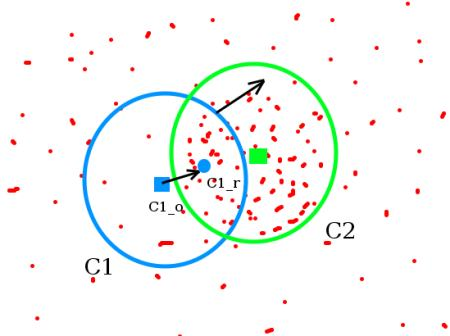
\includegraphics[scale=0.5 ]{meanshift.jpg}
			\centering
			\caption{  }
		\end{figure}
	 
  \item  The initial window is shown in blue circle with the name “C1”. Its original center is marked in blue rectangle, named “C1.o”. But if you find the centroid of the points inside that window, you will get the point “C1.r” (marked in small blue circle) which is the real centroid of window. Surely they don’t match. So move your window such that circle of the new window matches with previous centroid. Again find the new centroid. Most probably,it won’t match. So move it again, and continue the iterations such that center of window and its centroid falls on the same location (or with a small desired error). So finally what you obtain is a window with maximum pixel distribution. It is marked with green circle, named “C2”.
  \newline
  \begin{figure}[h!]
 \begin{subfigure}{0.5\textwidth}
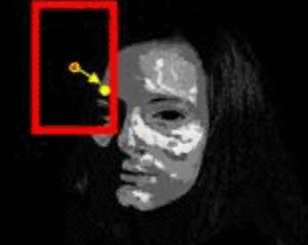
\includegraphics[width=0.9\linewidth, height=5cm]{mc1.png} 
\caption{Mean calculation}
\end{subfigure}
\begin{subfigure}{0.5\textwidth}
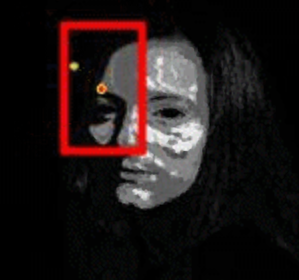
\includegraphics[width=0.9\linewidth, height=5cm]{ms1.png}
\caption{Mean shift}
\end{subfigure}
 \caption{Mean shift in first iteration}
\end{figure}
\begin{figure}[h!]
 \begin{subfigure}{0.5\textwidth}
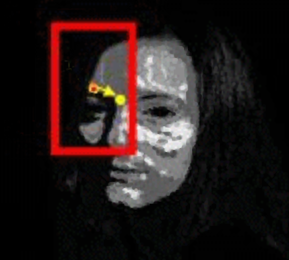
\includegraphics[width=0.9\linewidth, height=5cm]{mc2.png} 
\caption{Mean calculation}
\end{subfigure}
\begin{subfigure}{0.5\textwidth}
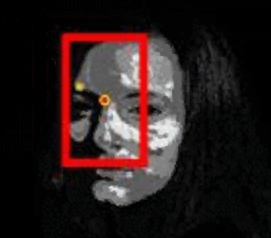
\includegraphics[width=0.9\linewidth, height=5cm]{ms2.png}
\caption{Mean shift}
\end{subfigure}
 \caption{Mean shift in second iteration}
\end{figure}
\begin{figure}[h!]
 \begin{subfigure}{0.5\textwidth}
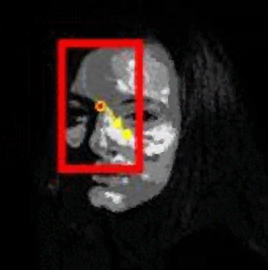
\includegraphics[width=0.9\linewidth, height=5cm]{mc3.png} 
\caption{Mean calculation}
\end{subfigure}
\begin{subfigure}{0.5\textwidth}
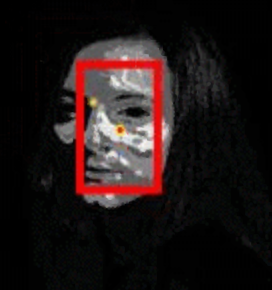
\includegraphics[width=0.9\linewidth, height=5cm]{ms3.png}
\caption{Mean shift}
\end{subfigure}
 \caption{Mean shift in third iteration}
\end{figure}
\begin{figure}[h!]
 \begin{subfigure}{0.5\textwidth}
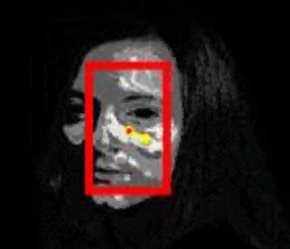
\includegraphics[width=0.9\linewidth, height=5cm]{mc4.png} 
\caption{Mean calculation}
\end{subfigure}
\begin{subfigure}{0.5\textwidth}
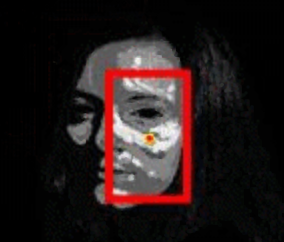
\includegraphics[width=0.9\linewidth, height=5cm]{ms4.png}
\caption{Mean shift}
\end{subfigure}
 \caption{Mean shift in fourth iteration}
\end{figure}
\begin{figure}[h!]
			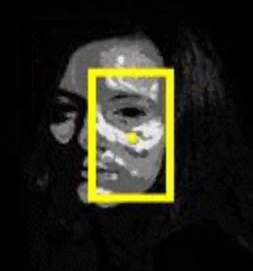
\includegraphics[scale=0.7]{convergedimage.png}
			\centering
			\caption{Converged Image}
		\end{figure}
\begin{figure}[h!]
			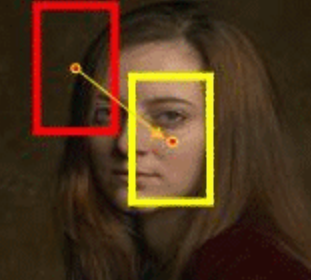
\includegraphics[scale=0.7]{shiftedwindow.png}
			\centering
			\caption{Shifted Window}
		\end{figure}\subsection{CAM Shift Algorithm}
		
\end{itemize}

  \begin{itemize}
     \item CAM Shift is an improvement of Mean shift algorithm known as Continously Adaptive Mean shift algorithm.It applies meanshift first.Once meanshift converges, it updates the size of the window. It also calculates the orientation of best fitting ellipse to it. Again it applies the meanshift with new scaled search window and previous window location. The process is continued until required accuracy is met.
    
    \item  It is almost same as meanshift, but it returns a rotated rectangle (that is our result) and box parameters (used to be passed as search window in next iteration).
     \item The Camshift cleverly exploits the algorithm of mean-shift by changing the size of the window when it happened to convergence. The Camshift coupled is an adaptation to the color image sequences, and is operated in pursuit of real-time object.
       \item CAMSHIFT was implemented as such:
   \begin{itemize}
   
\item Initial location of the 2D search window was computed.
\item  The color probability distribution is calculated for a region slightly bigger than the mean shift search window.
\item  Mean shift is performed on the area until suitable 
convergence. The zeroth moment and centroid coordinates are computed and stored.
\item  The search window for the next frame is centered around the centroid and the size is scaled by a function of the zeroth movement.
\item Reapeats again from step 2
\newline
\end{itemize}	
\end{itemize}

 \begin{figure}[h!]
 \begin{subfigure}{0.5\textwidth}
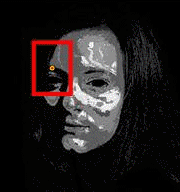
\includegraphics[width=0.9\linewidth, height=3.8cm]{msi.png} 
\caption{Meanshift 1st iteration}
\end{subfigure}
\begin{subfigure}{0.5\textwidth}
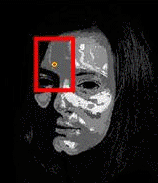
\includegraphics[width=0.9\linewidth, height=3.8cm]{ms2nd.png}
\caption{Meanshift 2nd iteration}
\end{subfigure}
\begin{subfigure}{0.5\textwidth}
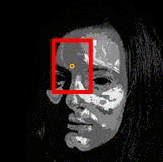
\includegraphics[width=0.9\linewidth, height=3.8cm]{ms3rd.png}
\caption{Meanshift 3rd iteration}
\end{subfigure}
\begin{subfigure}{0.5\textwidth}
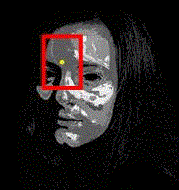
\includegraphics[width=0.9\linewidth, height=3.8cm]{msconverged.png} 
\caption{Converged  Meanshift}
\end{subfigure}
 \caption{Meanshift}
\end{figure}
 \begin{figure}[h!]
 \begin{subfigure}{0.5\textwidth}
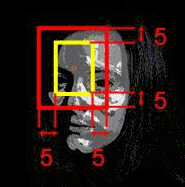
\includegraphics[width=0.9\linewidth, height=3.8cm]{roiforellipse.png}
\caption{Calculation of roi}
\end{subfigure}
\begin{subfigure}{0.5\textwidth}
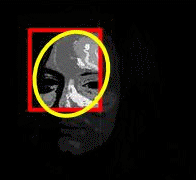
\includegraphics[width=0.9\linewidth, height=3.8cm]{ellipsecomputation.png}
\caption{Ellipse computation}
\end{subfigure}
\begin{subfigure}{0.5\textwidth}
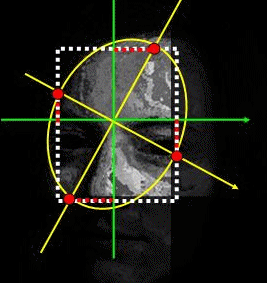
\includegraphics[width=0.9\linewidth, height=3.8cm]{newmeanshiftaxis.png} 
\caption{New meanshift axis}
\end{subfigure}
\begin{subfigure}{0.5\textwidth}
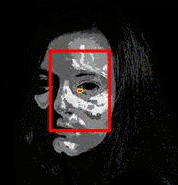
\includegraphics[width=0.9\linewidth, height=3.8cm]{meanshiftagain.png}
\caption{Meanshift again}
\end{subfigure}
 \caption{ellipse computation and applying Meanshift again}
\end{figure}
 \begin{figure}[h!]
 \begin{subfigure}{0.5\textwidth}
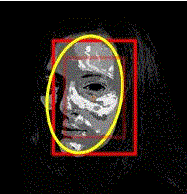
\includegraphics[width=0.9\linewidth, height=3.8cm]{msec.png} 
\caption{Ellipse calculation}
\end{subfigure}
\begin{subfigure}{0.5\textwidth}
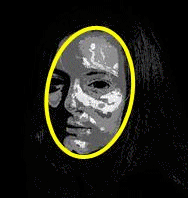
\includegraphics[width=0.9\linewidth, height=3.8cm]{convergedellipse.png}
\caption{Converged Ellipse}
\end{subfigure}
 \caption{Converged ellipse calcualtion}
\end{figure}

  \begin{figure}[h!]
 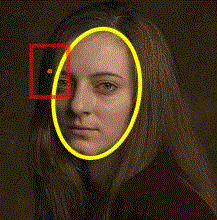
\includegraphics[width=0.9\linewidth, height=6cm]{result.png}
   \centering
 \caption{Resulting Camshift}
  \end{figure}

\end{itemize}	
 \newpage
 
\section{Experiment}
	The Python code using OpenCV and Numpy is given below.
	\newline
	\newline
	\lstinputlisting[language=Python]{Colored_Object_tracking_based_on_ROI_selection.py}
	\subsection{Mean Shift Code}
	 In Mean Shift we use the MeanShift function available in opencv.It is as follows:
	  \begin{figure}[h!]
 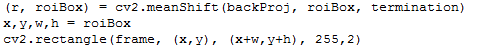
\includegraphics[scale=0.9]{meanshift.png}
   \centering
  \end{figure}
	\section{Exercise}
	Real time object tracking in a sample video  is shown below.          
	 \begin{figure}[h!]
 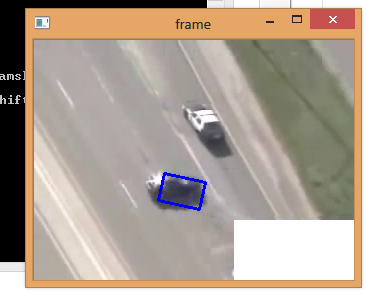
\includegraphics[scale=0.9]{Vid_ROI.png}
   \centering
 \caption{Selecting suspect car in a chase as ROI}
  \end{figure}
  \begin{figure}[h!]
 \includegraphics[scale=0.9]{Vid_Det.png}
   \centering
 \caption{Tracking the suspect in the frame}
  \end{figure}
  \newpage
 Real time object tracking in a webcam is shown below.  
	 \begin{figure}[h]
 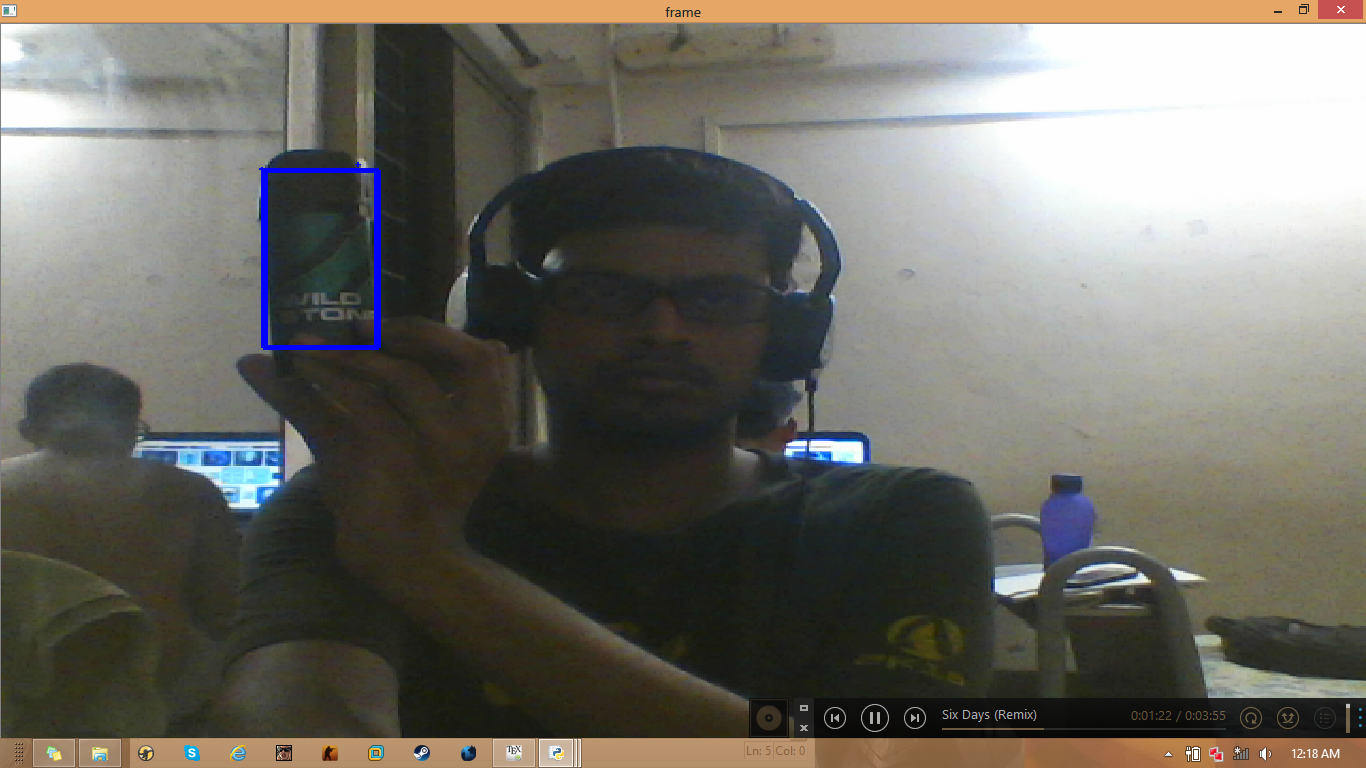
\includegraphics[width=0.9\linewidth, height=6.8cm]{Cam_ROI.png}
   \centering
 \caption{Selecting Deodrant as ROI}
  \end{figure}
  \begin{figure}[h]
 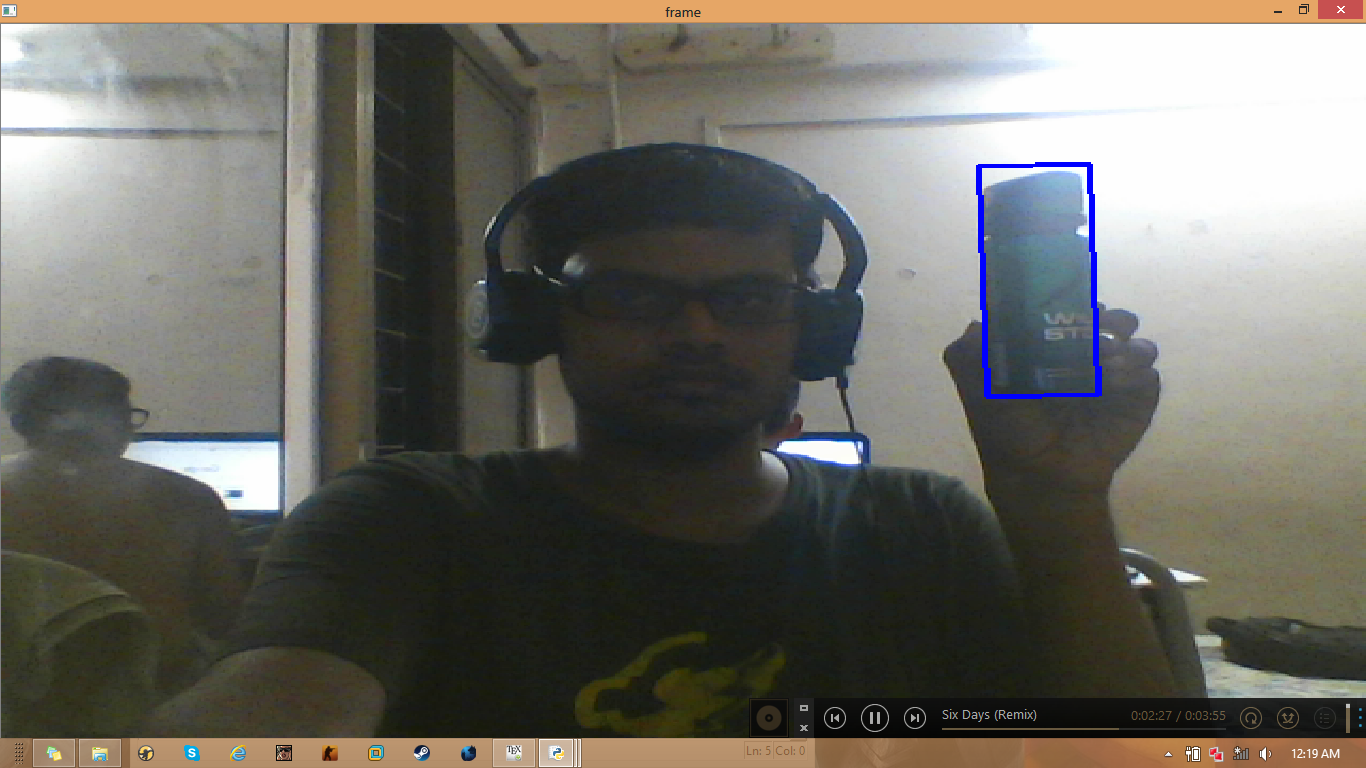
\includegraphics[width=0.9\linewidth, height=6.8cm]{Cam_Det.png}
   \centering
 \caption{Tracking the Deodrant in the frame}
  \end{figure}
	
	\newpage
	\section{References}
		\begin{enumerate}
			\item \url{http://opencv-python-tutroals.readthedocs.io/en/latest/py_tutorials/py_video/py_meanshift/py_meanshift.html#meanshift}
			\item \url{http://www.bogotobogo.com/python/OpenCV_Python/python_opencv3_mean_shift_tracking_segmentation.php}
			\item \url{http://www.computervisiononline.com/blog/tutorial-using-camshift-track-objects-video}
			\item \url{https://sites.google.com/a/ualberta.ca/jinxin-he/programming/python/simpleobjecttracking}
			\item \url{http://www.pyimagesearch.com/2015/05/25/basic-motion-detection-and-tracking-with-python-and-opencv/}
		\end{enumerate}
			
\end{document}



